\section{HỆ SỐ GÓC CỦA ĐƯỜNG THẲNG}
\subsubsection{Kiến thức trọng tâm}
\begin{itemize}
	\item Đường thẳng $y = ax + b \ (a \neq 0)$ có hệ số góc là $a$.
	\item Nếu $a > 0$, đường thẳng đi lên từ trái sang phải, góc tạo bởi đường thẳng này với trục $Ox$ là góc nhọn. 
	\item Nếu $a < 0$, đường thẳng đi xuống từ trái sang phải, góc tạo bởi đường thẳng này với trục $Ox$ là góc tù.
	\item Vị trí tương đối của hai đường thẳng $(d_1) \colon y = a_1x + b_1$, $(d_2) \colon y = a_2x + b_2$:
	\begin{itemize}
		\item $(d_1)$ và $(d_2)$ song song khi $a_1 = a_2$, $b_1 \neq b_2$.
		\item $(d_1)$ và $(d_2)$ trùng nhau khi $a_1 = a_2$, $b_1 = b_2$.
		\item $(d_1)$ và $(d_2)$ cắt nhau khi $a_1 \neq a_2$.
	\end{itemize}
\end{itemize}

\begin{vd}%[Dự án 9-EX-Đề Cương Toán 9]%[Mai Suong-087]%%[8D3N4-3]
	Xác định hệ số góc của đường thẳng $y = -2x + 1$. Cho biết đường thẳng đó tạo với trục $Ox$ góc nhọn hay góc tù?
	\loigiai{
		Đường thẳng $y = - 2x + 1$ có hệ số góc là $a=-2<0$ nên có góc tạo với trục $Ox$ là góc tù.
	}
\end{vd}

\begin{vd}%[Dự án 9-EX-Đề Cương Toán 9]%[Mai Suong-087]%%[8D3N4-5]
	Xét vị trí tương đối của các cặp đường thẳng sau
	\begin{enumerate}
		\item $d \colon y = 2x + 1$ và $d' \colon y = 2x - 3$.
		\item $d \colon y = -x + 2$ và $d' \colon y = x + 1$.
		\item $d \colon y = \dfrac{1}{2}x - 1$ và $d' \colon y = 0{,}5x - 1$.
	\end{enumerate}
	\loigiai{
		\begin{enumerate}
			\item $d \parallel d'$ (vì chúng có cùng hệ số góc là $2$ và khác tung độ gốc $1 \ne -3$).
			\item $d$ và $d'$ cắt nhau (vì chúng có hệ số góc khác nhau, $-1 \ne 1$).
			\item $d$ và $d'$ trùng nhau nhau (vì chúng có cùng hệ số góc là $\dfrac{1}{2}$ và cùng tung độ gốc $-1$).
		\end{enumerate}
	}
\end{vd}

\subsubsection{Bài tập}

\begin{bt}%[Dự án 9-EX-Đề Cương Toán 9]%[Mai Suong-087]%%[8D3N4-3]
	Tìm hệ số góc của đường thẳng sau
	\begin{multicols}{2}
		\begin{enumerate}
			\item $y = 3x - 5$;
			\item $y = -3x - 4$;
			\item $y = x$;
			\item $y = -x + \dfrac{3}{4}$.
		\end{enumerate}
	\end{multicols}
	\loigiai{
		\begin{enumerate}
			\item Đường thẳng $y = 3x - 5$ có hệ số góc $a = 3$.
			\item Đường thẳng $y = -3x - 4$ có hệ số góc $a = -3$.
			\item Đường thẳng $y = x$ có hệ số góc $a = 1$.
			\item Đường thẳng $y = -x + \dfrac{3}{4}$ có hệ số góc $a = -1$.
		\end{enumerate}
	}
\end{bt}


\begin{bt}%[Dự án 9-EX-Đề Cương Toán 9]%[Mai Suong-087]%%[8D3H4-3]
	Tìm hàm số bậc nhất có đồ thị là đường thẳng $d$ đi qua điểm $A(1;-2)$ và có hệ số góc là $3$.
	\loigiai{
		Đường thẳng $d$ có hệ số góc là $3$ nên nên hàm số bậc nhất có dạng $y=3x+b$.\\
		Đường thẳng $d$ đi qua điểm $A(1;-2)$ nên ta có 
		\begin{eqnarray*}
			-2 &=& 3 \cdot 1 + b\\
			-2 &=& 3 + b\\
			b &=& -5.
		\end{eqnarray*}
		Vậy hàm số cần tìm là $y=3x-5$.
	}
\end{bt}

\begin{bt}%[Dự án 9-EX-Đề Cương Toán 9]%[Mai Suong-087]%%[8D3N4-5]
	Xét vị trí tương đối của các cặp đường thẳng sau
	\begin{multicols}{2}
		\begin{enumerate}
			\item $y = x + 2$ và $y = -x + 2$;
			\item $y = 2x - 1$ và $y = 2x + 3$;
			\item $y = -3x + 1$ và $y = 4x - 2$;
			\item $y = \dfrac{1}{2}x + 1$ và $y = \dfrac{1}{2}x - 3$;
			\item $y = -2x + 5$ và $y = -2x + 1$;
			\item $y = \dfrac{3}{4}x - 1$ và $y = -\dfrac{3}{4}x + 2$.
		\end{enumerate}
	\end{multicols}
	\loigiai{
		\begin{enumerate}
			\item Đường thẳng $y = x + 2$ có hệ số góc $a = 1$, tung độ gốc $b = 2$.\\
			Đường thẳng $y = -x + 2$ có hệ số góc $a' = -1$, tung độ gốc $b' = 2$.\\
			Vì $a \ne a'$ nên hai đường thẳng này \textbf{cắt nhau}.
			\item Đường thẳng $y = 2x - 1$ có hệ số góc $a = 2$, tung độ gốc $b = -1$.\\
			Đường thẳng $y = 2x + 3$ có hệ số góc $a' = 2$, tung độ gốc $b' = 3$.\\
			Vì $a = a'$ và $b \ne b'$ nên hai đường thẳng này \textbf{song song}.
			\item Đường thẳng $y = -3x + 1$ có hệ số góc $a = -3$, tung độ gốc $b = 1$.\\
			Đường thẳng $y = 4x - 2$ có hệ số góc $a' = 4$, tung độ gốc $b' = -2$.\\
			Vì $a \ne a'$ nên hai đường thẳng này \textbf{cắt nhau}.
			\item Đường thẳng $y = \dfrac{1}{2}x + 1$ có hệ số góc $a = \dfrac{1}{2}$, tung độ gốc $b = 1$.\\
			Đường thẳng $y = \dfrac{1}{2}x - 3$ có hệ số góc $a' = \dfrac{1}{2}$, tung độ gốc $b' = -3$.\\
			Vì $a = a'$ và $b \ne b'$ nên hai đường thẳng này \textbf{song song}.
			\item Đường thẳng $y = -2x + 5$ có hệ số góc $a = -2$, tung độ gốc $b = 5$.\\
			Đường thẳng $y = -2x + 1$ có hệ số góc $a' = -2$, tung độ gốc $b' = 1$.\\
			Vì $a = a'$ và $b \ne b'$ nên hai đường thẳng này \textbf{song song}.
			\item Đường thẳng $y = \dfrac{3}{4}x - 1$ có hệ số góc $a = \dfrac{3}{4}$, tung độ gốc $b = -1$.\\
			Đường thẳng $y = -\dfrac{3}{4}x + 2$ có hệ số góc $a' = -\dfrac{3}{4}$, tung độ gốc $b' = 2$.\\
			Vì $a \ne a'$ nên hai đường thẳng này \textbf{cắt nhau}.
		\end{enumerate}
	}
\end{bt}


\begin{bt}%[Dự án 9-EX-Đề Cương Toán 9]%[Mai Suong-087]%%[8D3H4-5]
	Cho hai đường thẳng $d_1 \colon y = x - 7$, $d_2 \colon y = -2x - 1$. 
	\begin{enumerate}
		\item Tìm tọa độ giao điểm của hai đường thẳng đã cho.
		\item Tìm $m$ để hai đường thẳng đã cho và đường thẳng $d_3 \colon y=mx+1 (m\ne 0)$ đồng quy.
	\end{enumerate}
	\loigiai{
		\begin{enumerate}
			\item Ta có phương trình hoành độ giao điểm của $d_1$ và $d_2$ là
			\begin{eqnarray*}
				x - 7 &=& -2x - 1 \\
				3x &=& 6 \\
				x &=& 2.
			\end{eqnarray*}
			Thay $x=2$ vào hàm số $y = x - 7$, ta có $y = -5$.\\
			Vậy $d_1$ và $d_2$ cắt nhau tại điểm $A(2;-5)$.
			\item Hai đường thẳng đã cho và đường thẳng $d_3 \colon y=mx+1 (m\ne 0)$ đồng quy khi $d_3$ đi qua giao điểm $A(2;-5)$ của hai đường thẳng $d_1$ và $d_2$.\\
			Thay $x=2$, $y=-5$ vào phương trình đường thẳng $d_3$, ta có
			$$-5=m \cdot 2 + 1 \text{ hay } m=-3 \text{ (thỏa mãn) }$$.
		\end{enumerate}
	}
\end{bt}

\begin{bt}%[Dự án 9-EX-Đề Cương Toán 9]%[Mai Suong-087]%%[8D3H4-6]
	Tìm hàm số bậc nhất có đồ thị là đường thẳng $d$
	\begin{enumerate}
		\item đi qua $M(2;-3)$ và song song với đường thẳng $d_1 \colon y=-2x+5$.
		\item có hệ số góc là $-5$ và cắt trục tung tại điểm có tung độ là $7$.
		\item song song với $d_2 \colon y=3x-4$ và đi qua giao điểm của hai đường thẳng $d_3 \colon y=\dfrac{4}{5}x+\dfrac{3}{5}$ và $d_4 \colon y=2x-3$.
	\end{enumerate}
	\loigiai{
		\begin{enumerate}
			\item Vì $d$ song song với $d_1$ nên hệ số góc của $d$ bằng $-2$.\\
			Gọi $d\colon y=-2x+b \quad (b \ne 5)$. Vì $d$ đi qua $M(2;-3)$ nên
			\begin{eqnarray*}
				-3 &=& -2\cdot 2 + b \\
				-3 &=& -4 + b \\
				b &=& 1 \quad \text{ (thỏa mãn) }.
			\end{eqnarray*}
			Vậy $d\colon y=-2x+1$.
			\item Hệ số góc $k=-5$ và cắt trục tung tại điểm có tung độ là $7$ nên $b=7$.\\
			Do đó $d\colon y=-5x+7$.
			\item 
			Phương trình hoành độ giao điểm $P$ của $d_3$ và $d_4$ là
			\begin{eqnarray*}
				\dfrac{4}{5}x+\dfrac{3}{5} &=& 2x-3 \\
				4x+3 &=& 10x-15 \\
				-6x &=& -18 \\
				x &=& 3.
			\end{eqnarray*}
			Khi $x=3$ thì $y=2\cdot 3 - 3 = 3$.\\
			Suy ra $P(3;3)$.\\ 
			Vì $d$ song song với $d_2 \colon y=3x-4$ nên phương trình đường thẳng của $d$ có dạng $y=3x+b \quad (b\ne -4)$.\\
			Và $d$ đi qua $P(3;3)$ nên ta có
			\begin{eqnarray*}
				3 &=& 3\cdot 3 + b \\
				3 &=& 9 + b \\
				b &=& -6 \text{ (thỏa mãn) }.
			\end{eqnarray*}
			Vậy $d\colon y=3x-6$.
		\end{enumerate}
	}
\end{bt}


\begin{bt}%[Dự án 9-EX-Đề Cương Toán 9]%[Mai Suong-087]%%[8D3H4-6]
	Viết phương trình các đường thẳng sau
	\begin{enumerate}
		\item Đường thẳng song song với $y = 2x + 1$, đi qua $M(0; -3)$.
		\item Đường thẳng đi qua $N(1; 2)$ và vuông góc với đường thẳng $y = -x + 4$.
	\end{enumerate}
	\loigiai{
		\begin{enumerate}
			\item Vì đường thẳng cần tìm song song với đường thẳng $y=2x+1$ nên có phương trình dạng $y=2x+b \quad (b \ne 1)$. \\
			Vì đường thẳng đó đi qua $M(0;-3)$ nên
			\begin{eqnarray*}
				-3 &=& 2\cdot 0 + b \\
				b &=& -3. \text{ (thỏa mãn)}
			\end{eqnarray*}
			Vậy phương trình đường thẳng cần tìm là $y=2x-3$.
			\item Vì đường thẳng cần tìm vuông góc với đường thẳng $y = -x + 4$ nên có phương trình dạng $y=x+b$. \\
			Vì đường thẳng đó đi qua $N(1; 2)$ nên
			\begin{eqnarray*}
				2 &=& 1 + b \\
				b &=& 1.
			\end{eqnarray*}
			Vậy phương trình đường thẳng cần tìm là $y=x+1$.
		\end{enumerate}
	}
\end{bt}

\begin{bt}%[Dự án 9-EX-Đề Cương Toán 9]%[Mai Suong-087]%%[8D3V4-7]
	\immini{
		Đồ thị trong hình bên được sử dụng để đổi đơn vị độ dài inch sang xentimét.
		\begin{enumerate}
			\item Xem đồ thị hãy cho biết $2$ inch, $3$ inch bằng khoảng bao nhiêu xentimét?
			\item Xác định hệ số góc của đồ thị là đường thẳng trong hình bên.
	\end{enumerate}}{
		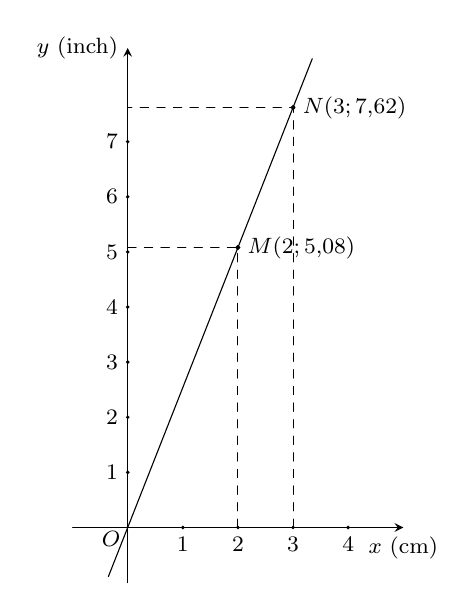
\begin{tikzpicture}[scale=0.7,font=\footnotesize, line join=round, line cap=round, >=stealth]
			\draw[-stealth](-1,0)--(5,0)node[below]{$x$ (cm)};
			\draw[-stealth](0,-1)--(0,8.7)node[left]{$y$ (inch)};
			\foreach \x in {1,2,3,4}{
				\fill (\x,0) node[below]{$\x$} circle(1pt);	}
			\foreach \y in {1,2,3,4,5,6,7}{
				\fill (0,\y) node[left]{$\y$} circle(1pt);}
			\node at (-0.3,-0.2) { \small \footnotesize $O$}; 
			\draw[samples=200,domain=-0.35:3.35]plot(\x,{2.54*(\x)});
			\draw[fill] (2,5.08) circle (1 pt)node[right]{\footnotesize $M(2;5{,}08)$};
			\draw[fill] (3,7.62) circle (1 pt)node[right]{\footnotesize $N(3;7{,}62)$};
			\draw[dashed] (2,0)--(2,5.08)--(0,5.08);
			\draw[dashed] (3,0)--(3,7.62)--(0,7.62);
		\end{tikzpicture}
	}
	\loigiai{
		\begin{enumerate}
			\item Theo đồ thị ta có: $2$ inch $\approx 5{,}08$ cm; \quad $3$ inch $\approx 7{,}62$ cm.
			\item Giả sử đường thẳng trong hình bên có dạng $y=ax+b$.\\
			Vì đường thẳng đi qua gốc tọa độ $O(0;0)$ nên $b=0$. Suy ra đường thẳng có dạng $y=ax$.\\
			Mặt khác, đồ thị đi qua điểm $M(2;5{,}08)$ nên ta có hệ số góc của đường thẳng là
			\begin{eqnarray*}
				5{,}08 &=& a\cdot 2 \\
				a &=& \dfrac{5{,}08}{2}=2{,}54.
			\end{eqnarray*}
		\end{enumerate}
	}
\end{bt}

\begin{bt}%[Dự án 9-EX-Đề Cương Toán 9]%[Mai Suong-087]%%[8D3V4-7]
	\immini{
		Đồ thị trong hình bên được sử dụng để đổi đơn vị độ dài dặm sang kilômét.
		\begin{enumerate}
			\item Xem đồ thị hãy cho biết $2$ dặm, $3$ dặm bằng khoảng bao nhiêu kilômét?
			\item Xác định hệ số góc của đồ thị là đường thẳng trong hình bên.
	\end{enumerate}}{
		\begin{tikzpicture}[scale=0.7,font=\footnotesize, line join=round, line cap=round, >=stealth]
			\draw[-stealth](-1,0)--(5,0)node[below]{$x \text{ (dặm)}$};
			\draw[-stealth](0,-1)--(0,7)node[left]{$y$ (km)};
			\foreach \x in {1,2,3,4}{
				\fill (\x,0) node[below]{$\x$} circle(1pt);	}
			\foreach \y in {1,2,3,4,5,6}{
				\fill (0,\y) node[left]{$\y$} circle(1pt);}
			\node at (-0.4,-0.2) { \small \footnotesize $O$}; 
			\draw[samples=200,domain=-0.5:4]plot(\x,{1.61*(\x)});
			\draw[fill] (2,3.22) circle (1 pt)node[right]{\footnotesize $M(2;3{,}22)$};
			\draw[fill] (3,4.83) circle (1 pt)node[right]{\footnotesize $N(3;4{,}83)$};
			\draw[dashed] (2,0)--(2,3.22)--(0,3.22);
			\draw[dashed] (3,0)--(3,4.83)--(0,4.83);
		\end{tikzpicture}
	}
	\loigiai{
		\begin{enumerate}
			\item Theo đồ thị ta có: $2$ dặm $\approx 3{,}22$ km; \quad $3$ dặm $\approx 4{,}83$ cm.
			\item Giả sử đường thẳng trong hình bên có dạng $y=ax+b$.\\
			Vì đường thẳng đi qua gốc tọa độ $O(0;0)$ nên $b=0$. Suy ra đường thẳng có dạng $y=ax$.\\
			Mặt khác, đồ thị đi qua điểm $M(2;3{,}22)$ nên ta có hệ số góc của đường thẳng là
			\begin{eqnarray*}
				3{,}22 &=& a\cdot 2 \\
				a &=& \dfrac{3{,}22}{2}=1{,}61.
			\end{eqnarray*}
		\end{enumerate}
	}
\end{bt}

\begin{bt}%[Dự án 9-EX-Đề Cương Toán 9]%[Mai Suong-087]%%[8D3V4-7]
	Chị Lan làm nghề bán nước giải khát. Chị nhận thấy số li nước chanh bán được trong ngày và nhiệt độ trung bình của ngày hôm đó có mối quan hệ tỉ lệ thuận với nhau. Chị đã ghi lại các giá trị tương ứng trong bảng sau:
	
	\begin{center}
		\begin{tabular}{|c|c|c|c|c|c|c|}
			\hline
			$x$ (°C) & 20 & 22 & 24 & 26 & 28 & 30 \\ \hline
			$y$ (li nước chanh) & 10 & 11 & 12 & 13 & 14 & 15\\ \hline
		\end{tabular}
	\end{center}
	
	\begin{enumerate}
		\item Hãy biểu diễn $y$ theo $x$.
		\item Tìm hệ số góc của đường thẳng là đồ thị của hàm số ở câu a).
	\end{enumerate}
	\loigiai{
		\begin{enumerate}
			\item Theo đề ta có $y$ và $x$ là hai đại lượng tỉ lệ thuận nên $y=ax$ và khi $x=20$ thì $y=10$.\\
			Suy ra $10=a \cdot 20$ hay $a=\dfrac{1}{2}$.\\ 
			Vậy $y=\dfrac{1}{2}x$.
			\item Hệ số góc của đường thẳng là $a=\dfrac{1}{2}$.
		\end{enumerate}
	}
\end{bt}

\begin{bt}%[Dự án 9-EX-Đề Cương Toán 9]%[Mai Suong-087]%%[8D3V4-7]
	Giá cho thuê nhà trọ của hai chủ nhà A và B như bảng sau:
	\begin{center}
		\begin{tabular}{|c|c|c|}
			\hline
			Chủ nhà & Tiền thuê nhà trọ và tiền nước mỗi tháng & Giá tính mỗi kWh điện \\
			\hline
			A & 500\,000 đồng & 2\,000 đồng \\
			\hline
			B & 450\,000 đồng & 2\,500 đồng \\
			\hline
		\end{tabular}
	\end{center}
	Gọi $x$ (kWh) là số điện tiêu thụ mỗi tháng của người thuê nhà; $y$ (đồng) là số tiền người thuê nhà phải trả trong mỗi tháng.
	\begin{enumerate}
		\item Viết công thức tính $y$ theo $x$ trong trường hợp một người thuê nhà của chủ nhà A. Công thức này có phải là hàm số bậc nhất không?
		\item Viết công thức tính $y$ theo $x$ trong trường hợp một người thuê nhà của chủ nhà B. Công thức này có phải là hàm số bậc nhất không?
		\item Trong trường hợp các công thức ở câu a) và b) là hàm số bậc nhất, hãy tìm vị trí tương đối của hai đường thẳng là đồ thị của hai hàm số đó.
		\item Khi nào thì số tiền người thuê nhà phải trả trong mỗi tháng cho chủ nhà A và chủ nhà B bằng nhau?
	\end{enumerate}
	\loigiai{
		\begin{enumerate}
			\item Với chủ nhà A: số tiền phải trả là
			$$y = 2\,000x + 500\,000.$$
			Đây là hàm số bậc nhất (vì có dạng $y = ax + b$ với $a \ne 0$).
			\item Với chủ nhà B: số tiền phải trả là
			$$y = 2\,500x + 450\,000.$$
			Đây cũng là hàm số bậc nhất.
			\item Ta có hai đường thẳng:
			$$d\colon y = 2\,000x + 500\,000, \quad d'\colon y = 2\,500x + 450\,000.$$
			Vì hệ số góc khác nhau ($2\,000 \ne 2\,500$) nên hai đường thẳng $d$ và $d'$ cắt nhau.
			\item Nếu số tiền phải trả cho hai chủ nhà bằng nhau thì
			$$2\,500x + 450\,000 = 2\,000x + 500\,000.$$
			Suy ra
			\begin{eqnarray*}
				2\,500x - 2\,000x &=& 500\,000 - 450\,000 \\
				500x &=& 50\,000 \\
				x &=& 100.
			\end{eqnarray*}
			Vậy khi người thuê nhà sử dụng $100$ kWh điện mỗi tháng thì số tiền phải trả cho chủ nhà A và B bằng nhau.
		\end{enumerate}
	}
\end{bt}
